\documentclass[11pt,a4j]{jsarticle}
\usepackage{url}
\usepackage{listings,jlisting}
\usepackage{comment}

 \usepackage{amsmath}
 \usepackage[amsmath,thmmarks]{ntheorem}

  \theorembodyfont{\normalfont}
\theoremstyle{plain}
\theoremseparator{.}
\theoremprework{\bigskip\hrule\bigskip}
\theorempostwork{\hrule\bigskip}
 \newtheorem{theo}{定理}[section]
 \newtheorem{defi}[theo]{定義}
 \newtheorem{lemm}[theo]{補題} 
 \renewcommand{\thetheo}{\arabic{theo}} 





%\usepackage{geometry}                % See geometry.pdf to learn the layout options. There are lots.
%\geometry{letterpaper}                   % ... or a4paper or a5paper or ... 
%\geometry{landscape}                % Activate for for rotated page geometry
%\usepackage[parfill]{parskip}    % Activate to begin paragraphs with an empty line rather than an indent
%\usepackage{graphicx}
%\usepackage{amssymb}
%\usepackage{epstopdf}
\usepackage[dvipdfmx]{graphicx}
\DeclareGraphicsRule{.tif}{png}{.png}{`convert #1 `dirname #1`/`basename #1 .tif`.png}



%Hyper Cube - Hn
%Star Graph - Sn
%Pancake Graph Pn
%Burnt Pancake Graph : BPn
%Half Pancake Graph HPn
%Rotator Graph : Rn
%Bi Rotator Graph : BRn
%Transposition Graph : Tn
%Substring Reversal Graph : SRn



\title{特別研究計画 }
\author{鄭 信雨\\学籍番号 11834304}
%\date{}                                           % Activate to display a given date or no date

\def\vector#1{\mbox{\boldmath $#1$}}
\def\O#1{\overline#1}

\begin{document}



\maketitle
\newpage
\tableofcontents
\newpage


 \section{はじめに}
このレポートは特別研究計画最終レポートである。
 \section{目的}
このレポートは今まで自身の研究のために調査してきた研究を簡潔にまとめ報告することを目的とする。
\section{背景}
逐次計算システムの性能向上の頭うちにより近年並列分散計算システムが様々な分野で活用されるようになってきた。
それと同時に並列分散処理計算システムの研究開発も活発に行われている\cite{top500}。
日本国内でも2012年11月スーパーコンピューター京が正式運用を開始したが、
その僅か4年後の2016年11月には京の浮動小数演算性能の約2.2倍高性能なOakforest-PACS スーパーコンピュータシステムが
正式運用を開始するなど、並列分散処理計算機システムの活発な研究開発を確認することができる\cite{kcomputer}\cite{oakforest}。

 並列分散性能に直接関連するのは各ノードの個別性能も重要であるが、ノード間の通信方式を決める位相もとても重要である。
例えば任意の二つのノード間で情報交換が必要になった場合なるべく短い経路で情報交換ができることが望ましい。
最も距離を短くするには全てのノードを隣接させることで可能にはなるが、数十万、数百万のノード間に全てリンクを設置するの現実的に不可能である。
また、並列分散計算システムでは耐故障生の確保もとても重要である。巨大な数のノードを扱うので運用上一部のノードの故障を避けることはできない\cite{diskfailures}。
しかし、並列分散計算システムではたとえ一部のノードが故障していても可能な限り正しく動作する必要がある。
この問題を解決するためにグラフ理論が用いられるようになった。
並列分散システムの各ノードを頂点としリンクを辺にすることでグラフ理論を用いることができる。
このような背景より並列分散システムの位相を与えることができる様々な相互結合網が提案されてきた。例えば、メッシュ や ハイパーキューブ、パンケーキなどがある。
そして、それらの相互結合網において耐故障経路選択解法や並列通信経路解法などが数多く提案されてきた。
本レポートでは相互結合網における耐故障性および並列通信経路の解法である頂点間、頂点と頂点集合間、頂点集合間、素な経路選択アルゴリズムに関する論文に関して
解説する。


\newpage

%諸定義
\documentclass[11pt,a4j]{jsarticle}
\usepackage{url}
\usepackage{listings,jlisting}
\usepackage{comment}
\usepackage{amsmath}
\usepackage[amsmath,thmmarks]{ntheorem}
\usepackage[dvipdfmx]{graphicx}
\theorembodyfont{\normalfont}
\theoremstyle{plain}
\theoremseparator{.}
\theoremprework{\bigskip\hrule\bigskip}
\theorempostwork{\hrule\bigskip}
\newtheorem{theo}{定理}[section]
\newtheorem{defi}[theo]{定義}
\newtheorem{lemm}[theo]{補題}
\renewcommand{\thetheo}{\arabic{theo}} 
\def\vector#1{\mbox{\boldmath $#1$}}
\def\vu{\mbox{\boldmath $u$}}
\def\vv{\mbox{\boldmath $v$}}

\def\node#1#2{\mbox{\boldmath $#1_{#2}$}}

\def\O#1{\overline#1}
\begin{document}



%諸定義
\section{諸定義}
本章では、本レポートで使用する用語の定義を行う。

%Graph
\begin{defi}
グラフ(graph)は頂点(vertex, node)を要素と持つ空でない集合と,二つの頂点を要素とする辺(edge, link)を要素と持つ集合からなる.頂点集合が$V$,辺集合が$E$であるグラフ$G$を$G$($V$,$E$)と書く.
\end{defi}

%directed / undirected  graph
\begin{defi}
各辺を定義する頂点の対が順序対であるとき,そのグラフを有向グラフ(directed graph),非順序対のとき,無向グラフ(undirected graph)と呼ぶ.
\end{defi}

%adjacent
\begin{defi}
二つの頂点{\vu}, {\vv}と辺$e$に対して,{\vu}, {\vv}$\in$, $e$のとき,$e$は{\vu}, {\vv}に接続しているという.また,{\vu} ,{\vv}は隣接している(adjacent),$e$の端点(end point)は{\vu} ,{\vv}である,という.以後,頂点{\vv}の隣接頂点集合を$N$({\vv})で表す.
\end{defi}

%isolated 
\begin{defi}
無向グラフの頂点{\vv}において,{\vv}に接続している辺の数を{\vv}の次数(degree)という.次数が0である頂点を孤立頂点(isolated vertex)という.
\end{defi}

%degree
\begin{defi}
無向グラフ$G$において,任意の頂点の次数のうち,最大のものを$G$の最大次数(maximum degree),最小のものを$G$の最小次数(minimum degree)と言う.
\end{defi}

%in,out degree
\begin{defi}
有向グラフの頂点{\vv}において, {\vv}から出る辺の集合を{\it out}({\vv}),{\vv}へ入る辺の集合を{\it in}({\vv})とする. $|{\it out}({\vv})|$, $|{\it in}({\vv})|$をそれぞれ{\vv}の出次数(out degree), 入次数(in degree)という. 出次数, 入次数が共に0である頂点を孤立頂点という.
\end{defi}

%regular graph
\begin{defi}
全ての頂点の次数が等しいグラフを正則グラフ(regular graph)と言う.
\end{defi}

%symmetric
\begin{defi}
グラフ$G$の任意の二頂点{\vu}, {\vv}に対し、{\vu}を{\vv}へ写す$G$の自己同型写像があるとき,$G$を頂点対称(vertex transitive, vertex symmetric)という.$G$の任意の二辺$e_1$, $e_2$に対し, $e_1$を$e_2$へ写す$G$への自己同型写像があるとき,$G$を辺対称(edge transitive, edge symmetric)という.
\end{defi}

%path
\begin{defi}
無向グラフ$G(V,E)$の$k$個の頂点の系列{\node v1}, {\node v2}, {\dots}, {\node vk}が $1\leq i \leq k - 1$となる$i$に対して({\node vi}, {\node v{i+1}}) $\in E$を満たすとき, この系列を$G$の{\node v1}から{\node vk}への長さ $k - 1$の経路(path)という. 有向グラフにおいては,有向経路(directed path)という. 
\end{defi}

%cycle
\begin{defi}
先頭の頂点と最後の頂点が同じ経路を閉路(cycle)という.
\end{defi}

%self loop
\begin{defi}
両端の頂点が同じ辺を自己閉路(self loop)という.
\end{defi}

%underlying graph
\begin{defi}
有向グラフ$G$において, 各辺の向きを無くして得られるグラフを$G$の基礎グラフ(underlying graph)という.
\end{defi}

%connected
\begin{defi}
任意の二頂点間に有向経路が存在する有向グラフを強連結(strongly connected)という. 任意の二頂点間に経路が存在する無向グラフを連結(connected)という. 
有向グラフは, その基礎グラフが連結であるとき, 連結という. 強連結でも連結でもないグラフを非連結(unconnected)という.
\end{defi}

%tree
\begin{defi}
閉路を含まない連結なグラフを木(tree)という.
\end{defi}

%multiple edge
\begin{defi}
無向グラフにおいて, 隣接するある二頂点間に複数の辺が存在するとき, これらの辺を多重辺(multiple edge)という. 有向グラフにおいて, 隣接するある二頂点{\vu , \vv}間に, 
{\vu}から{\vv}への複数の辺が存在する場合, これらの辺を多重辺という.
\end{defi}

%simple graph
\begin{defi}
自己閉路と多重辺を持たないグラフを単純グラフ(simple graph)という.
\end{defi}

%shortest path
\begin{defi}
グラフ$G$の二頂点{\vu , \vv} 間の経路のうち, 長さが最も短いものを$G$における{\vu , \vv}間の最短経路(shortest path)という.
\end{defi}

%distance
\begin{defi}
二頂点{\vu , \vv}間の最短経路の長さを{\vu , \vv}間の距離(distance)という. {\vu , \vv}間に経路が存在しない場合は, {\vu , \vv}間の距離を$\infty$とする.
\end{defi}

%diameter
\begin{defi}
連結グラフ$G$の任意の二頂点間の距離のうち, 最大のものを$G$の直径(diameter)という. 以降グラフ$G$の直径を$D(G)$で表す.
\end{defi}

%subgraph
\begin{defi}
グラフ$G(V,E)$に対し, 次の条件を全て満たすグラフ$G'(V', E')$を$G$の部分グラフ(subgraph)という.
\begin{itemize}
\item $V' \subseteq V$
\item $E' \subseteq E$
\end{itemize}
\end{defi}


%subtree
\begin{defi}
部分グラフのうち, 木であるものを部分木(subtree)という.
\end{defi}

%spanning tree
\begin{defi}
グラフ$G$の部分木のうち, その頂点が$G$のすべての頂点からなるものを$G$の全域木(spanning tree)という.
\end{defi}

%connectivity
\begin{defi}
連結なグラフ$G$に対して, 以下の二つの条件をともに満たす最小の$k$を$G$の連結度(connectivity)という.
\begin{itemize}
\item $G$の任意の$k - 1$個の頂点を取り除いたグラフは連結である.
\item $G$のある$k$個の頂点を取り除いたグラフが非連結に, あるいはたったひとつの頂点からなるグラフになる.
\end{itemize}
\end{defi}

%k-connected
\begin{defi}
連結度が$k$であるグラフを$k$-連結($k$-connected)という.
\end{defi}


%disjoint path
\begin{defi}
複数の経路が頂点を共有しないとき, これらの経路を互いに素な経路(disjoint path)という.
\end{defi}

%internally-disjoint paths /  node-to-node disjoint paths
\begin{defi}
二頂点{\vu , \vv}を結ぶ複数の経路が{\vu , \vv}を除いて頂点を共有しないとき, これらの経路を内素な経路(internally-disjoint paths)もしくは
頂点間素な経路(node-to-node disjoint paths)という.
\end{defi}

%node-to-set disjoint paths
\begin{defi}
頂点{\vu}と{\vu}を含まない頂点集合{$V$}を結ぶ複数の経路が{\vu}を端点とした場合を除いて頂点を共有しないとき,これらの経路を頂点と頂点集合間素な経路(node-to-set disjoint paths)という.
\end{defi}

%set-to-set disjoint paths
\begin{defi}
頂点{\node v1 ,\dots , \node vn}を要素として持つ集合$V$と$V$の頂点を含まない
頂点{\node u1 ,\dots , \node un}を要素として持つ集合$U$ に対して{\node ui, \node vj ($1\leq i,j \leq n$)}間を結ぶ複数の経路が頂点を共有しないとき,これらの経路を頂点集合間素な経路(set-to-set disjoint paths)という.
\end{defi}

%Group
\begin{defi}
集合$B$に演算$\circ $が定義されていて次の性質を全て満たす時, $\langle B,\circ\rangle$を群(group)という.
\begin{itemize}
\item $B$の任意の元$x,y,z$に対して,\[ (x\circ y)\circ z = x\circ(y\circ z)\]を満たす.
\item $B$の任意の元$x$に対して,\[ x\circ e = e\circ x = x \]を満たす$B$の元$e$が存在する.この$e$を群$\langle B,\circ\rangle$の単位元(unit element, identity)という.
\item $B$の任意の元$x,y,z$に対して,\[ x\circ x^{-1} = x^{-1}\circ x = e\]を満たす$B$の元$x^{-1}$が存在する.
\end{itemize}
\end{defi}

%generator set
\begin{defi}
$B = \langle B,\circ\rangle$を群とし, $B$の元の部分集合を$X$とする.$B$の任意の元を$X$の元と演算$\circ$の組み合わせで表すことができるとき, $X$ を$B$の生成元集合(generator set)という.
\end{defi}

%directed cayley graph
\begin{defi}
$B = \langle B,\circ\rangle$を群,$X$を$B$の生成元集合とする. 有向グラフ$C*(B,X)$は, その頂点集合$V(C*(B,X))$と辺集合$E(C*(B,X))$をそれぞれ
\begin{equation*} 
	\begin{split}
	V(C*(B,X)) &= B \\
	E(C*(B,X)) &= \{\{b,x\circ b\}| b \in B, x \in X\} 
	\end{split}
\end{equation*}
とするとき, 有向ケイリーグラフと呼ばれる.
\end{defi}


%cayley graph
\begin{defi}
$B = \langle B,\circ\rangle$を群,$X$を$B$の生成元集合とする. 
$X$の任意の要素$x$に対して$x^{-1}\in X$であるとする. 無向グラフ$C(B,X)$は
その頂点集合$V(C*(B,X))$と辺集合$E(C*(B,X))$をそれぞれ
\begin{equation*} 
	\begin{split}
	V(C*(B,X)) &= B \\
	E(C*(B,X)) &= \{\{b,x\circ b\}| b \in B, x \in X\} 
	\end{split}
\end{equation*}
とするとき, ケイリーグラフと呼ばれる.
\end{defi}






\end{document}

\begin{defi}

\end{defi}





%グラフの比較を行う。
%静的ルーティング
%動的ルーティングに関して述べる。






\section{スターグラフ}
この節では、スターグラフに関する主な性質および有用な経路選択アルゴリズムに関する論文を紹介する。


\subsection{スターグラフの定義}
$s_1s_2\dots s_n$を$1$から$n$までの$n$種類の記号で作られる順列とする。$SWAP_j(s_1s_2\dots s_n)=s_js_2\dots s_{j-1}s_1s_{j+1}\dots s_n$と定義する。
無向グラフ$G(V,E)$に対して$n$-star graph $S_n=(V,E)$は$V=\{(u_1u_2\dots u_n)|(u_1u_2\dots u_n)は1,2,\dots ,nの順列\}$と$E=\{(u,SWAP_i(u) | u \in V, 2 \leq i \leq n )\}$である。


\subsection{スターグラフの性質}
スターグラフは再帰性と対称性をグラフでハイパーキューブに代わる位相として注目を集めている。表\ref{tab:sn_prop}にスターグラフの性質を示す。

\begin{table}[htb]
  \begin{center}
    \caption{$n$-スターグラフの性質}
    \begin{tabular}{|c|c|c|c|} \hline
      頂点数&次数&連結度&直径 \\ \hline 
      $n!$ & $n-1$&$n-1$& $\lfloor3(n - 1) /2 \rfloor$ \\ \hline
    \end{tabular}
        \label{tab:sn_prop}
  \end{center}
\end{table}

\begin{figure}
\centering
  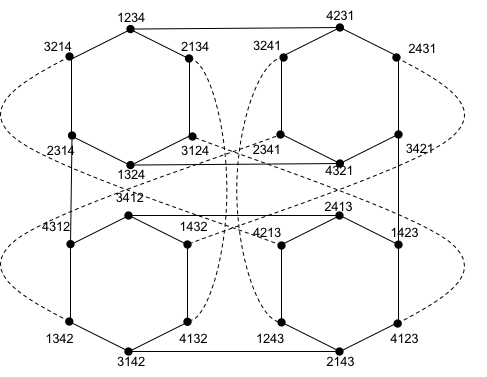
\includegraphics[width=\linewidth]{stargraph.png}
 \caption{$3$,$4$ - Star graph}
\label{fig:stargraph}
\end{figure}




\subsection{スターグラフ関連研究紹介}
%Selection, Routing, and Sorting on the Star Graph \UTF{2217}%
\subsubsection{Selection, Routing, and Sorting on the Star Graph}
この節ではスターグラフにおけるSelection、Routing、Sortingに関してより効率的な解法を論文 \cite{star-routing}に関して述べる。\newline
Sortingは与えられた順列を昇順、もしくは降順に並べかえる工程である。\newline
Routingはパケット情報を出発地点より目的地点まで送ることである。\newline
この論文ではまず記号列に対するPrefix computationを$O(n^2)$で達成する解法を提案する。
実際にスターグラフにおけるPrefix computationの最適な時間計算量は$O(nlogn)$ですでに提案されている\cite{star-optimal-prefix-computation}が
本論文で提案された解法は並列処理が可能になるように工夫されているため、$n$個の記号列に対するPrefix computationも$O(n^2)$で可能であることを提案している。
このPrefix computationの解法を彼らの他の解法のサブルーチンとして活用している。この解法を用いることで$n$-スターグラフでのSortingを$O(n^3)$で実現している。
また、Selectionに関しては$O(n^2)$でRoutingに関しては$O(n^3)$での解法を提案している。特にRoutingに関しては既知の解法は$O(n^3logn)$であること比べ改善されている。
これは彼らが提案したPrefix computationの解法が並列処理をした場合$O(n^2)$で解決できるため、既存の$O(n^2logn)$より改善されたためである。





\begin{comment}
We present an algorithm that performs a sequence of n prefix computations in O(n2) time. This
algorithm is used as a subroutine in our other algorithms. We also show that sorting can be performed
on the n-star graph in time O(n3) and that selection of a set of uniformly distributed n keys can be
performed in O(n2) time with high probability. Finally, we also present a deterministic (non oblivious)
routing algorithm that realizes any permutation in O(n3) steps on the n-star graph.
There exists an algorithm in the literature that can perform a single prefix computation in O(n lg n)
time. The best known previous algorithm for sorting has a run time of O(n3 lg n) and is deterministic.
To our knowledge, the problem of selection has not been considered before on the star graph.

Before our work, the best known sorting algorithm for the n-star graph ran in O(n3 lg n) time [7, 2]. A
different algorithm with the same run time has been given in [15]. Whereas [7, 2]’s algorithm is based on
shearsort, [15]’s algorithm is based on bitonic sort and the underlying constant is also small (i.e., 1
2 ). We present an improved sorting algorithm which runs on the n-star graph in O(n3) time with high probability.
Our approach to randomized sorting differs from previous approaches in that we use repeated selection. These
algorithms make use of prefix and selection algorithms that we have designed. Our selection algorithm can
perform a set of n selections in O(n2) time with high probability provided the keys to be selected have ranks
uniform in the interval [1, n!]. The prefix algorithm presented in this paper can compute the prefixes of n
different sequences in O(n2) time. In contrast, Akl and Qiu [2] show that a single prefix computation can
be performed in O(n lg n) time, which is the best possible. Prefix computation is performed using a tree
like subgraph (which we call as a ‘(k, 1, k) chain network’). This network, we believe, is applicable for many
other computations as well. Similar networks have been used before [7, 2].
Efficient packet routing algorithms for the star graph have already been obtained in [9]. Although the
best known randomized routing algorithm for the star graph runs in O(n) time with very high probability
[9], due to the lower bound of [5], the best known deterministic oblivious routing algorithm for the star graph
needs a much higher running time. In this paper we develop a non-oblivious deterministic routing algorithm
with O(n3) running time.
\end{comment}

\subsubsection{Node-to-node cluster fault tolerant routing in star graphs}
この節ではスターグラフにおける頂点間耐クラスタ故障ルーティングアルゴリズムに関する研究 \cite{star-n2n}を紹介する。
ここでクラスタ故障とは、故障頂点の集合である。$n$-スターグラフは$n$-1の次数を持つ正則グラフであるため、$n-1$の連結度を持つ。
メンガーの定理により$n$-グラフでは高々$n-2$子の任意の故障頂点に耐えることができるがこの論文ではさらに直径が高々$2$である高々$n-2$の
クラスタ故障に対して非故障出発頂点と目的頂点間に経路を構築する手法を提案している。
この提案手法は最大経路長が$\lfloor3(n - 1) /2 \rfloor +8$である場合計算量が$O(|クラスタ| + n)$であり、
最大経路長が$\lfloor3(n - 1) /2 \rfloor +6$である場合計算量が$O(n^2)$である。
提案手法のキーポイントは$n$-スターグラフが$n$個の$n-1$-スターグラフを含んでいる再帰的な構造を利用している。
論文では、頂点順列の最右記号$k( 1 \leq k \leq n )$が同じである順列より誘発される$n-1$-サブスターグラフにを$k$-サブグラフとする。
そして、$i$-サブグラフ内部より長さが高々$2$以下で$j$-サブグラフに移動する頂点集合を $i$より$j$へのポート集合として定義している。
このようなポート集合は任意の$k$-サブグラフ内部に$n-1$個存在する。本論文ではこのポート集合を活用し頂点間耐クラスタ故障ルーティング手法を
提案している。


\subsubsection{Node-to-set disjoint paths problem in star graphs}
この節ではスターグラフにおける頂点と頂点集合間の素な経路選択問題に関する二つの解法を提案した論文\cite{star-n2s}に関して述べる。\newline
スターグラフにおける頂点と頂点集合間の素な経路選択問題は\cite{star-n2s-first}で最初に解法が提案された。
\cite{star-n2s-first}で提案された手法は$n$-スターグラフ内の$n-1$の素な経路を構築するのに$O(n^2)$の時間計算量を必要とし、経路長は最大$5(n-2)$であった。
これに対し本論文で提案された手法では時間計算量は同じであるが、最大経路長が$\lfloor3(n - 1) /2 \rfloor +3$である{\it simple algorithm}と$\lfloor3(n - 1) /2 \rfloor +2$ である
{\it refined simple algorithm}を提案した。{\it simple algorithm}は大きく二つのサブルーチン{\it SCATTER}と{\it MERGE-THEN-REDUCE}で構成されている。{\it SCATTER}では与えられた順列組に対して記号1を先頭に持ってくる作業を行う。
この作業で得られた結果はすべて素な経路になる。例えば{\it SCATTER}([13241, [4321], [3421])により次の三つの素な経路が構築される。$P_1 : v_1 = t_l = [1324], P_2 : [4321] \rightarrow  [2341] \rightarrow	 v2 = [1342], P_3 : [3421] \rightarrow v_3 = [1423].$\newline 
$n$-スターグラフ内の複数の頂点ペア間の最短経路はお互い素でない可能性がある。
しかし、本論文で提案されている二つ目のサブルーチン{\it MERGE-THEN-REDUCE}では一定の条件を満たす頂点集合と出発頂点間で互いに素な最短経路を構築することができる。
この{\it MERGE-THEN-REDUCE}が{\it simple algorithm}で構築された$n-1$個の経路が互いに素であるための重要な役割を果たしている。\newline
最後に{\it simple algorithm}より最大経路長が1少ない{\it refined simple algorithm}は{\it simple algorithm}で最初に行われる{\it SCATTER}操作時に検知される最悪のケースに対して再度経路を改善することを実装している。






\section{バブルソートグラフ}


\section{トランスポジショングラフ}
この節では、トランスポジショングラフに関する主な性質および有用な経路選択アルゴリズムに関する研究を紹介する。


\subsection{トランスポジショングラフの定義}
$s_1s_2\dots s_n$を$1$から$n$までの$n$種類の記号で作られる順列とする。$TP_{(i,j)}(s_1s_2\dots s_n)=s_1s_2\dots s_{i-1}s_{j}s_{i+1}\dots s_{j-1}s_{i}s_{j+1}\dots s_n$と定義する。
無向グラフ$G(V,E)$に対して$n$-トランスポジショングラフ $T_n=(V,E)$は$V=\{(u_1u_2\dots u_n)|(u_1u_2\dots u_n)は1,2,\dots ,nの順列\}$と$E=\{(u,TP_{(i,j)}(u) | u \in V, 1 \leq i < j \leq n)\}$である。


\subsection{トランスポジショングラフの性質}
トランスポジショングラフは再帰性と対称性を持つグラフで表\ref{tab:tn_prop}のような性質を持つ。

\begin{table}[htb]
  \begin{center}
    \caption{$n$-トランスポジショングラフの性質}
    \begin{tabular}{|c|c|c|c|} \hline
      頂点数&次数&連結度&直径 \\ \hline 
      $n!$ & $n(n-1)/2$&$n(n-1)/2$& $n-1$\\ \hline
    \end{tabular}
        \label{tab:tn_prop}
  \end{center}
\end{table}

\subsection{トランスポジショングラフの関連研究紹介}
\subsubsection{Node-disjoint paths in a transposition graph}
本論文\cite{tp-n2s}では$n$-トランスポジショングラフの頂点と頂点集合間素な経路選択問題に関する解法を提案している。
提案された手法は$0(n^7)$の時間計算量を必要とし、最大経路長は$3n-5$である。\newline
$n$-トランスポジショングラフの次数は$n(n-1)/2$であり、これは構築が必要な素な経路が$n(n-1)/2$個必要であることを意味する。
そして、提案手法のキーポイントはグラフの再帰構造を利用している点である。
$n$-トランスポジショングラフは頂点順列の最右記号$k( 1 \leq k \leq n )$が同じである順列より誘発される$n-1$-サブトランスポジショングラフ
$n$個に分割することができる。トランスポジショングラフは対称性を持っているため、出発頂点$s$を$12\dots n$に固定することができる。
これに対して任意の目的頂点の数を$n(n-1)/2$とする。経路構築のために出発頂点が存在する$n-1$サブトランスポジショングラフの中に目的頂点が
いくつ存在するかによって場合を分ける。出発頂点と同一サブグラフの中に$(n-1)(n-2)/2$個以上が存在する場合その目的頂点を長さ高々2の経路で
他のサブグラフへ送り出す。もし、$(n-1)(n-2)/2$個以下存在する場合は他のサブグラフに存在する目的頂点を出発頂点が存在するサブグラフへ持ってくる。
この操作を全ての経路が構築されるまで繰り返す。

\subsubsection{Polynomial time algorithm for constructing vertex-disjoint paths in transposition graphs}
本論文\cite{tp-n2s2}では$n$-トランスポジショングラフの頂点と頂点集合間素な経路選択問題に関する解法を提案している。
該当問題はすでに\cite{tp-n2n}で解決されたが提案された手法とは違うアプローチを取ることで、問題の解決に要する時間計算量を$O(n^6)$に減らし
最大経路長も高々最短経路長+6に減らしている。\newline
この論文で提案された手法のキーポイントはグラフの頂点に対してVerticalクラスタリング及びHorisontalクラスタリングを行なったことと、
クラスタリングされた頂点間を2部グラフとみなし、2部グラフにおける極大マッチングを行っでいることである。

\section{パンケーキグラフ}
この節では、パンケーキグラフ関する主な性質および有用な経路選択アルゴリズムに関する研究を紹介する。


\subsection{パンケーキグラフの定義}
$s_1s_2\dots s_n$を$1$から$n$までの$n$種類の記号で作られる順列とする。$PR_{(i)}(s_1s_2\dots s_n)=s_is_{i-1}\dots s_1s_{i+1}s_{i+2}\dots s_n$と定義する。
無向グラフ$G(V,E)$に対して$n$-パンケーキグラフ $P_n=(V,E)$は$V=\{(u_1u_2\dots u_n)|(u_1u_2\dots u_n)は1,2,\dots ,nの順列\}$と$E=\{(u,PR_{(i)}(u) | u \in V, 2 \leq u \leq n)\}$である。
以後$n$-パンケーキグラフグラフを$P_n$とする。

\subsection{パンケーキグラフの性質}
パンケーキグラフは再帰性と対称性を持つグラフで表\ref{tab:tn_prop}のような性質を持つ。
\begin{table}[httpb]
  \begin{center}
    \caption{$n$-パンケーキグラフの性質}
    \begin{tabular}{|c|c|c|c|} \hline
      頂点数&次数&連結度&直径 \\ \hline 
      $n!$ & $n-1$&$n-1$& $$\\ \hline
    \end{tabular}
        \label{tab:pn_prop}
  \end{center}
\end{table}
\subsection{パンケーキグラフの関連研究紹介}
\subsubsection{An Algorithm for Node-Disjoint paths in Pancake graphs}
本論文\cite{pan-n2n}では$P_n$における頂点間素な経路選択問題に関する解法を提案している。
提案手法の時間計算量は$O(n^3)$であり、最大経路長は??である。
提案手法ではグラフの対称性利用し出発頂点${\vector s}$を$12\dots n$に固定する。
次に目的頂点$\vector{d}$によって次の3つのケースに分ける。
\begin{description}
 \item[Case 1] $\vector{d} = d_1d_2\dots d_{n-1}n$
 \item[Case 2]  $\vector{d} = nd_1d_2\dots d_{n}$
 \item[Case 3]  $Otherwise.$
\end{description}
素な経路を構築するアルゴリズムのキーポイントはグラフの再帰構造を利用することである。
頂点順列の最右記号$k( 1 \leq k \leq n )$が同じである順列より誘発される$n-1$-部分パンケーキグラフを$P_{n-1}(k)$とする。
Case 1の場合は出発頂点と目的頂点が$P_{n-1}(n)$に属している状態である。
部分グラフ内で構築できる最大の素な経路は$n-2$個であるため、異なる部分グラフを利用し出発頂点と目的頂点を連結するパスを構築後、
出発頂点と目的頂点が含まれている部分パンケーキグラフでアルゴリズムを再帰的に適用し$n-2$個の経路を構築する。Case 2の場合は
$PR_n(\vector{d})$と出発頂点\vector {s}と出発頂点が存在する部分パンケーキグラフ内で1本の経路を構築後$n-2$個の\vector{s}の隣接頂点を
$n-2$個の$P_{n-1}(k) (2 \leq k \le n)$他のサブグラフへ移動する経路を構築し、さらにそれぞれのサブグラフより$P_{n-1}(n)$に移動する経路を
構築する。これにより、\vector{d}が属している部分パンケーキグラフで、再度再帰的に提案手法を適用することができる。Case 3では Case 2のような$P_{n-1}(s)$より
$\vector{d}$へ直接いく経路($\vector{d}$以外$P_{n-1}(d)$の頂点が経路に含まれない)が存在しないため$P_{n-1}(d_1)$の頂点を利用し直接いく経路を1個mn構築する。
それ以降はCase 2とほぼ同じく$n-2$個の$\vector{s}$の隣接頂点を他の部分パンケーキグラフを利用し$\vector{d}$が属している部分グラフへの$n-2$個の経路を構築することで
\vector{d}が属している部分パンケーキグラフで、再度再帰的に提案手法を適用することができる。

\subsubsection{Node-to-Set Disjoint Paths Problem in Pancake Graphs}
本論文\cite{pan-n2s}ではパンケーキグラフにおける頂点と頂点集合間素な経路選択問題に関する解法を提案している。
提案手法の時間計算量は$O(n^5)$であり、最大経路長は??である。
提案手法のキーポイントは$P_n$の各頂点を$PR_{n-1},PR_{n}$を交互に適用しすることで得られるクラスに分類したことである。
この分類による各クラスは以下の4つの重要な特徴を持つ。

\begin{enumerate}
 \item 各頂点は必ず一つのクラスに属する。
 \item 各クラスには2$n$個の頂点が存在し、リング構造である。
 \item 各$P_(n-1)$には同じクラスの頂点がちょうと2個存在する。
 \item 各頂点は同じクラスに属する二つの隣接頂点を持ち、異なるクラスに属する$(n-3)$個の隣接頂点を持つ。
\end{enumerate}

例えば$P_4$の全ての頂点は以下の3つのクラスに分類できる。
\begin{description}
\item {C1} = {(1,2,3,4),(4,3,2,1),(2,3,4,1),(1,4,3,2), (3,4,1,2),(2,1,4,3),(4,1,2,3),(3,2,1,4)}
\item {C2} = {(2,1,3,4),(4,3,1,2),(1,3,4,2),(2,4,3,1), (3,4,2,1),(1,2,4,3),(4,2,1,3),(3,1,2,4)}
\item {C3} = {(1,3,2,4),(4,2,3,1),(3,2,4,1),(1,4,2,3), (2,4,1,3),(3,1,4,2),(4,1,3,2),(2,3,1,4)}
\end{description}
本論文\cite{pan-n2s}の提案手法は二つの手順で構成されている。
手順1は全ての目的頂点が$P_{n-1}(n)$に属している特別な場合を扱っている。この手順では$n-2$個の素な経路提案手法を再帰的に適用することでを$P_{n-1}(n)$で構築したあと、
残り1本の経路を$P_{n-1}(n)$以外のサブグラフで構築すしている。
手順2は手順1の場合以外の一般的な場合を扱っている。最初$P{n_1}(n)$に含まれている$n-1$個の頂点より、すべての目的頂点への素な経路を先ほど提案したclassの経路を利用し構築する。
その後、経路の一部を修正し出発頂点へつなぎ直す。最後に提案手法を再帰的に適用し全体のパスを構築する。


\section{焦げたパンケーキグラフ}
この節では、焦げたパンケーキグラフ関する主な性質および有用な経路選択アルゴリズムに関する研究を紹介する。
\subsection{焦げたパンケーキグラフ}
$s_1s_2\dots s_n$を$1$から$n$までの$n$種類の記号で作られる符号付き順列とする。符号付き前置反転操作$SR_{(i)}(s_1s_2\dots s_n)=\overline{s_is_{i-1}}\dots \overline{s_1}s_{i+1}s_{i+2}\dots s_n$と定義する。
無向グラフ$G(V,E)$に対して$n$-焦げたパンケーキグラフ $BP_n=(V,E)$は$V=\{(u_1u_2\dots u_n)|(u_1u_2\dots u_n)は符号付き1,2,\dots ,nの順列\}$と$E=\{(u,PR_{(i)}(u) | u \in V, 2 \leq u \leq n)\}$である。
以後$n$-焦げたパンケーキグラフを$BP_n$とする。

\subsection{焦げたパンケーキグラフの性質}
パンケーキグラフは再帰性と対称性を持つグラフで表\ref{tab:tn_prop}のような性質を持つ。
\begin{table}[httpb]
  \begin{center}
    \caption{$n$-焦げたパンケーキグラフの性質}
    \begin{tabular}{|c|c|c|c|} \hline
      頂点数&次数&連結度&直径 \\ \hline 
      $n!\times 2^n$ & $n-1$&$n-1$&\\ \hline
    \end{tabular}
        \label{tab:bpn_prop}
  \end{center}
\end{table}


%焦げたパンケーキグラフの関連研究紹介
\subsection{焦げたパンケーキグラフの関連研究紹介}

%焦げたパンケーキグラフN2S
\subsubsection{An Algorithm for Node-to-Set Disjoint Paths Problem in Burnt Pancake Graphs}
本論文\cite{bpn-n2s}では焦げたパンケーキグラフにおける頂点と頂点集合間素な経路選択問題に関する解法を提案している。
提案手法の時間計算量は$O(n^5)$であり、最大経路長は??である。
提案手法のキーポイントは$BP_n$の各頂点に対して$SR_n$と$SR_{n-1}$を交互に適用することで得られる頂点集合を{\it Traversal class}と定義しその性質を利用していることである。{\it Traversal class}では次の重要な性質を持つ。
\begin{enumerate}
 \item 各頂点は必ず一つのクラスに属する。
 \item 各クラスには4$n$個の頂点が存在し、リング構造である。
 \item 各$BP_(n-1)$には同じクラスの頂点がちょうと2個存在する。
 \item 各頂点は同じクラスに属する二つの隣接頂点を持ち、残りの隣接頂点は異なるクラスに属する。
\end{enumerate}
たとえば、$BP_3$は次の4つの{\it Traversal class}が存在する。
\begin{description}
\item 
$\begin{aligned}[b] {C1} = \{& (1, 2, 3), (\O3, \O2, \O1), (2, 3, \O1),  (1, \O3, \O2),(3, \O1, \O2), (2, 1, \O3),\\
    	 				 & (\O1, \O2, \O3), (3, 2, 1),(\O2, \O3, 1), (\O1, 3, 2), (\O3, 1, 2),   (\O2, \O1, 3)  \}
\end{aligned}$

\item 
$\begin{aligned}[b] {C2} = \{&(\O2, 1, 3), (\O3, \O1, 2), (1, 3, 2), (\O2, \O3, \O1),(3, 2, \O1), (1, \O2, \O3),\\
					  &(2, \O1, \O3), (3, 1, \O2),(\O1, \O3, \O2), (2, 3, 1), (\O3, \O2, 1), (\O1, 2, 3)\}
\end{aligned}$

\item 
$\begin{aligned}[b] {C3} = \{&(\O1, \O2, 3), (\O3, 2, 1), (\O2, 3, 1), (\O1, \O3, 2),(3, 1, 2), (\O2, \O1, \O3),\\
					 & (1, 2, \O3), (3, \O2, \O1),(2, \O3, \O1), (1, 3, \O2), (\O3, \O1, \O2), (2, 1, 3)\}
\end{aligned}$

\item 
$\begin{aligned}[b] {C4} = \{&(2, \O1, 3), (\O3, 1, \O2), (\O1, 3, \O2), (2, \O3, 1),(3, \O2, 1), (\O1, 2, \O3),\\
					  &(\O2, 1, \O3), (3, \O1, 2),(1, \O3, 2), (\O2, 3, \O1), (\O3, 2, \O1), (1, \O2, 3)\}
\end{aligned}$
\end{description}
$BP_n$の頂点と頂点集合間の素な経路選択アルゴリズムは
1.すべての目的頂点が出発頂点と同じ部分グラフ$BP_{n-1}(n)$に属している場合と、
2.1以外の場合に分けて解法を提案している。
1の場合では$BP_{n-1}(n)$で提案手法を再帰的に適用し、$n-1$個の素な経路を構築する。
そして、残りの1本の経路を$BP_{n-1}(n)$以外の部分グラフを用いて経路を構築する。
2の場合ではすべての目的頂点グループを$BP_{n-1}(n)${\it Traversal class}上に存在し、かつ他の目的頂点を
含まない場合$D1$とそうでない場合に$D2$わける。分けられたグループに対して、$D1$はそのまま出発頂点への経路を構築し
$D2$に対しては、{\it Traversal class}上で目的頂点の経路上での重複が避けられるように経路を再構築しながら出発頂点への経路を構築する。



\newpage
\section{まとめ}
 \section{おわりに}
  
  \newpage
 \begin{comment}
シェアソート
シェアソート(英: shear-sort)は、ソートのアルゴリズムの一つ。シェアソートでは、データを長方形に並べた上で、各行/各列ごとにソートを行なう。1989年に Isaac D. Scherson らが発表した[1]。安定ではない内部ソートであり、最悪の場合の時間計算量はO(n1.5)である。各行/各列の比較は互いに独立であるため、バブルソートとは異なり、並列動作が可能である。

Deterministic Oblivious Routing
http://algo.rwth-aachen.de/Lehre/SS12/VTDS/oblivious(1).pdf

インターコネクション技術
http://www.ieice-hbkb.org/files/06/06gun_05hen_09.pdf

残余ネットワーク
http://even-eko.hatenablog.com/entry/2013/08/08/195120
\end{comment}
  
\begin{thebibliography}{9}
\bibitem{top500}Top 500, https://www.top500.org/lists/2016/11/, Jan. 2017.
\bibitem{kcomputer}Mitsuo Yokokawa, et al. "The K computer: Japanese next-generation supercomputer development project, " {\it Low Power Electronics and Design (ISLPED) 2011 International Symposium on. IEEE}, 2011.
\bibitem{oakforest}Oakforest-PACS スーパーコンピュータシステム, http://www.cc.u-tokyo.ac.jp/system/ofp/, Jan. 2017.
\bibitem{diskfailures}Disk failures in the real world: What does an MTTF of 1,000,000 hours mean to you?, https://www.usenix.org/legacy/events/fast07/tech/schroeder/schroeder\_html/index.html, Jan.2017.


\bibitem{star-routing} Sanguthevar Rajasekaran and David S. L. Wei, "Selection, Routing, and Sorting on the Star Graph,	"  {\it Journal of Parallel and Distributed Computing}, {vol.42},{no.2},pp225-233, 1997.
\bibitem{star-optimal-prefix-computation}S.G. Akl and K. Qiu, "Data Communication and Computational Geometry on the Star and Pancake Interconnection Networks," {\it Parallel and Distributed Processing, 1991. Proceedings of the Third IEEE Symposium}, pp415-422,1991.
\bibitem{star-n2n} Qian-Ping Gu and Shietung Peng , "Node-to-node cluster fault tolerant routing in star graphs," {\it Information Processing Letters}, {vol.56},pp29-35, 1995.
\bibitem{star-n2s-first} M. Dietzfelbinger, S. Madhavapeddy and I.H. Sudborough, "Three disjoint path paradigms in star networks,"  {\it Proc. IEEE Symp. on Parallel and Distribured Processing} ,pp400-406, 1991.
\bibitem{star-n2s} Qian-Ping Gu and Shietung Peng , "Node-to-set disjoint paths problem in star graphs,"  {\it Information Processing Letters}, {vol.62},pp201-207, 1996.
\bibitem{tp-n2n}S. Latifi and P. K. Srimani, "Transposition networks as a class of fault-tolerant robust networks,'" {\it IEEE Transactions on Computers},{vol.45, no.2}, pp230-238, 1996.
\bibitem{tp-n2s}Y. Suzuki, K. Kaneko and M. Nakamori, "Node-disjoint paths in a transposition graph," {\it Proceedings of the International Conference on Parallel and Distributed, Processing Techniques and Applications},pp. 298-304,  2004. 
\bibitem{tp-n2s2}Satoshi Fujita, "Polynomial time algorithm for constructing vertex-disjoint paths in transposition graphs," {\it Networks}, Volume 56,  pp. 149-157, September 2010. 
\bibitem{pan-n2n} , Keiichi Kaneko, and Yasuto Suzuki, "An Algorithm for Node-Disjoint Paths in Pancake Graphs," {\it IEICE Trans. Information and Systems}, Vol. E86-D, No. 3, pp. 610-615, Mar. 2003
\bibitem{pan-n2s} Keiichi Kaneko, and Yasuto Suzuki, "Node-to-Set Disjoint Paths Problem in Pancake Graphs," {\it IEICE Trans. Information and Systems}, Vol. E86-D, No. 9, pp. 1628-1633, Sept. 2003.
\bibitem{bpn-n2s}Keiichi Kaneko, "An Algorithm for Node-to-Set Disjoint Paths Problem in Burnt Pancake Graphs," {\it IEICE Transactions on Information and Systems}, Vol. E86-D, No. 12, pp. 2588-2594, Dec. 2003


\end{thebibliography}






.\end{document}  